\documentclass[conference]{IEEEtran}
\IEEEoverridecommandlockouts
% The preceding line is only needed to identify funding in the first footnote. If that is unneeded, please comment it out.
\usepackage{cite}
\usepackage{amsmath,amssymb,amsfonts}
\usepackage{algorithmic}
\usepackage{graphicx}
\usepackage{textcomp}
\usepackage{xcolor}
\usepackage{hyperref}
\def\BibTeX{{\rm B\kern-.05em{\sc i\kern-.025em b}\kern-.08em
    T\kern-.1667em\lower.7ex\hbox{E}\kern-.125emX}}
\begin{document}

\title{Learning Reflections: Glass Facades for Urban-Scale - Final Report\\
% {
% \footnotesize 
% \textsuperscript{*}Note: Sub-titles are not captured in Xplore and should not be used}
% \thanks{Identify applicable funding agency here. If none, delete this.}
}

\author{\IEEEauthorblockN{Shin Li}
\IEEEauthorblockA{
% \textit{} \\
\textit{Rice University}\\
Houston, TX \\
zl186@rice.edu}
\and
\IEEEauthorblockN{Chi Xu}
\IEEEauthorblockA{
% \textit{} \\
\textit{Rice University}\\
Houston, TX \\
cx31@rice.edu}
\and
\IEEEauthorblockN{Yunan Wang}
\IEEEauthorblockA{
% \textit{} \\
\textit{Rice University}\\
Houston, TX \\
yw256@rice.edu}
\and
\IEEEauthorblockN{Yixing Liu}
\IEEEauthorblockA{
% \textit{} \\
\textit{Rice University}\\
Houston, TX \\
yl366@rice.edu}
\and
\IEEEauthorblockN{Wentao Jiang}
\IEEEauthorblockA{
% \textit{} \\
\textit{Rice University}\\
Houston, TX \\
wj30@rice.edu}
}
\maketitle

\begin{abstract}
Glass buildings and mirror-like surfaces in urban environments create complex reflections that challenge existing 3D reconstruction systems. Traditional methods often treat reflections as noise, leading to incorrect geometry and incomplete reconstructions in glass-rich environments. Current reflection-aware approaches mainly focus on avoiding reflective regions or separating reflection layers in 2D images, but they fail to recover accurate 3D geometry. This project aims to develop a reflection-aware 3D reconstruction framework that transforms reflections from obstacles into valuable sensing information. By combining geometric surface recovery of glass facades with machine learning–based reflection modeling, our approach enables simultaneous reconstruction of true building geometry and extraction of environmental information from reflected imagery. 


\end{abstract}

\begin{IEEEkeywords}
Reflection-aware reconstruction, glass facades, 3D geometry recovery, reflection modeling, machine learning
\end{IEEEkeywords}

% \section{Introduction}
% The growing use of glass in modern urban architecture creates visually striking yet technically challenging scenes for computer vision and 3D reconstruction. Unlike diffuse surfaces, glass produces complex mirror-like reflections that distort the apparent geometry of surrounding environments. When captured by cameras or LiDAR \cite{sadeghi20153d}, these reflections often lead to ghost structures, incorrect depth estimation, and incomplete reconstructions.

% Conventional reconstruction methods—such as SfM, MVS, and SLAM—assume Lambertian surfaces, where appearance does not depend on viewing direction. This assumption fails for reflective and transparent materials, causing reflections to be treated as artifacts and resulting in missing data and reduced accuracy for urban-scale modeling. Recent reflection-aware approaches, like separating reflection and transmission layers or avoiding reflective regions in SLAM, focus on discarding reflections rather than leveraging them, limiting accurate 3D reconstruction of glass surfaces and extraction of environmental information from reflections \cite{klimkowska2022detailed}.

% Early reflection reconstruction studies approached the problem from a geometric perspective. Hu et al. \cite{hu2005mirror} demonstrated that a planar mirror can serve as a virtual camera, enabling multi-view 3D reconstruction of reflected objects through geometric constraints between real and virtual views. Similarly, Kanbara et al. \cite{kanbara2006spherical} employed a spherical mirror to capture multiple reflections from different directions for reconstructing the 3D structure of reflected scenes. These mirror-based approaches revealed that reflections can encode geometric information of the surrounding environment; however, they rely on idealized mirror assumptions, strict calibration, and controlled laboratory setups. Such methods fail to generalize to non-planar or semi-transparent glass surfaces that exhibit spatially varying normals and complex, distorted reflections commonly observed in urban facades.

% With the rise of neural scene representations, recent methods have shifted from geometric modeling to data-driven reasoning. NeRF \cite{nerf} provides the foundational neural radiance field formulation, but its standard rendering process struggles with mirror-like reflections because view-dependent appearance and true geometry are highly entangled. To address these limitations, several NeRF variants have introduced reflection-aware mechanisms, including the decomposition strategies used in NeRFReN \cite{guo2022nerfren} and the specular ray-tracing formulation employed in TraM-NeRF \cite{holland2024tramnerf}, which together provide improved handling of reflective surfaces compared to vanilla NeRF. Recently, the Visual Geometry Grounded Transformer (VGGT) \cite{wang2025vggt} introduced a large feed-forward transformer capable of jointly predicting camera parameters, depth, point maps, and 3D tracks from multi-view inputs in a single forward pass. Although not specifically tailored for reflective scenes, VGGT demonstrates strong generalization across complex 3D perception tasks, providing a promising foundation for reflection-aware geometry estimation. Compared with these methods, our work bridges geometric modeling and neural representations by leveraging both synthetic and real-world data to learn how reflections encode surface geometry and environmental context, ultimately enabling more accurate 3D reconstruction in glass-rich environments.

% Our goal is to move beyond reflection removal by leveraging reflections as informative cues for 3D reconstruction. We model the physical formation of reflections on glass surfaces and learn to interpret reflected content to jointly recover façade geometry and surrounding environments. In our work, we develop a Mitsuba-based simulation pipeline that generates physically realistic reflective scenes for model training and evaluation, complemented by real-world camera data for validation. This reflection-aware framework integrates geometric modeling with learning-based neural network reflection interpretation, providing the foundation for the method described in the following section.



\section{Introduction}
Glass surfaces in modern urban architecture pose significant challenges for computer vision and 3D reconstruction. Unlike diffuse materials, glass produces mirror-like reflections that distort apparent geometry. These reflections cause ghost structures, incorrect depth estimation, and incomplete reconstructions in camera and LiDAR data \cite{sadeghi20153d}.

Traditional reconstruction methods, like SfM, MVS, and SLAM, assume Lambertian surfaces with view-independent appearance. This assumption fails for reflective materials, causing reflections to be treated as artifacts, reducing accuracy in urban-scale modeling. Current reflection-aware approaches focus on suppressing or avoiding reflections rather than exploiting them, limiting both glass surface reconstruction and environmental information extraction \cite{klimkowska2022detailed}.
Early geometric methods demonstrated reflection utility. Hu et al. \cite{hu2005mirror} showed that planar mirrors act as virtual cameras for multi-view reconstruction, while Kanbara et al. \cite{kanbara2006spherical} used spherical mirrors to capture multiple reflections. However, these approaches require idealized conditions and controlled setups, failing to generalize to non-planar, semi-transparent glass with spatially varying normals and distorted reflections, which are common in urban facades.

Neural scene representations offer new possibilities. While NeRF \cite{nerf} struggles with reflections due to entangled view-dependent appearance and geometry, variants like NeRFReN \cite{guo2022nerfren} and TraM-NeRF \cite{holland2024tramnerf} improve handling through decomposition and specular ray-tracing. The Visual Geometry Grounded Transformer (VGGT) \cite{wang2025vggt} jointly predicts camera parameters, depth, and 3D structure in a single forward pass, demonstrating strong generalization across complex perception tasks. Our work bridges geometric modeling and neural methods by learning how reflections encode surface geometry and environmental context.

Rather than removing reflections, we leverage them as informative cues. We model reflection formation on glass and learn to interpret reflected content to recover both façade geometry and surrounding environments. Our Mitsuba-based simulation pipeline generates physically realistic reflective scenes for training, validated against real-world data. This framework integrates geometric principles with neural reflection interpretation, providing the foundation for our method.

\section{Method}

\subsection{Baseline: COLMAP SfM/MVS Reconstruction}

As our classical 3D reconstruction baseline, we adopt COLMAP \cite{schonberger2016structure}, a widely used open-source pipeline for Structure-from-Motion (SfM) and Multi-View Stereo (MVS) on unstructured image collections. COLMAP first runs incremental SfM: SIFT feature extraction and matching \cite{lowe2004distinctive}, geometric verification, and bundle adjustment to recover camera poses and a sparse 3D point cloud. It then performs dense multi-view stereo, using PatchMatch-based depth estimation \cite{schonberger2016pixelwise} and depth-map fusion to produce a dense 3D point cloud or mesh. This two-stage pipeline is a strong off-the-shelf choice on standard, mostly Lambertian scenes.

In glass-rich urban environments, however, the key assumptions of COLMAP are systematically violated. Glass façades are non-Lambertian: strong, view-dependent reflections break photo-consistency and lead to ghost geometry, where reflected buildings or interiors are reconstructed as floatinenables COLMAP to handle datasets ranging from small objects to entire cities, comprising outliers, leaving holes or missing façades. Texture sparsity, repetitive patterns, and specular highlights further degrade feature matching, causing fragmented reconstructions or pose failures.

In experiments, we treat COLMAP as a glass-agnostic baseline operating directly on RGB images, without any explicit handling of reflective regions. The failure modes of this baseline motivate the second component of our method, a learning-based glass segmentation module (GEM; Section~\ref{sec:gem}), providing façade masks to downstream reconstruction instead of treating all reflection-induced measurements as noise.


\subsection{GEM: Glass Surface Segmentation Models}
\label{sec:gem}
Accurate glass region identification is critical for reflection-aware reconstruction, enabling targeted processing of reflective surfaces while preserving non-reflective elements. We employ GEM \cite{hao2025gem}, which leverages vision foundation models for robust glass segmentation without task-specific fine-tuning. Traditional methods struggle with glass surfaces due to their lack of distinctive features and variable appearance depending on context and reflections, particularly in complex urban scenes with diverse architectural elements.

GEM adapts pre-trained vision foundation models, Segment Anything Model (SAM) and Grounding DINO, through a lightweight architecture preserving their visual priors \cite{kirillov2023segment,liu2024grounding}. The method generates glass-relevant prompts via CLIP-based similarity matching, guides Grounding DINO to produce candidate bounding boxes, and refines them into pixel-precise masks using SAM. A trainable fusion module (2.4M parameters) aggregates multi-scale features from frozen foundation models, distinguishing glass from visually similar surfaces while maintaining efficiency. In our pipeline, GEM masks delineate regions where standard MVS assumptions fail, provide spatial priors for normal and depth estimation, and establish a complete chain from raw imagery to reflection-aware 3D reconstruction.


\subsection{Normal Map Estimation from Distorted Reflections}

To study how small surface deformations affect reflection geometry, we implemented a normal map computation pipeline inspired by Jacquet \textit{et al.}~\cite{jacquet2013real}. Their work demonstrated that by tracking curved reflections of real-world straight lines on nearly planar glass surfaces, one can recover local surface normals through quadratic constraints and global smoothness optimization. In our setting, we replicate this principle within a controlled simulation using Mitsuba~3.

Specifically, we construct a nearly planar reflective surface with known perturbations defined by a smooth height function $h(x,y)$, producing local normal vectors:
\[
\mathbf{n}(x,y)=\frac{(-\partial h/\partial x,\,-\partial h/\partial y,\,1)}{\sqrt{(\partial h/\partial x)^2+(\partial h/\partial y)^2+1}}.
\]
A moving virtual camera scans the reflective surface while capturing reflections of structured patterns or linear features, producing a synthetic video analogous to the real-world setup in~\cite{jacquet2013real}. Each frame contains both RGB images and corresponding ground-truth normal maps. This simulation enables controlled evaluation of normal-estimation algorithms by comparing analytical normals from the height field with those inferred from reflection cues. The resulting dataset further supports training reflection-aware reconstruction models to predict surface orientation from reflected patterns.


\subsection{VGGT-Based Mirror Correction}

While the Visual Geometry Grounded Transformer (VGGT) effectively recovers dense 3D geometry from monocular inputs, it inherently adheres to a "line-of-sight" principle. Consequently, specular surfaces such as mirrors are reconstructed as virtual images located deep behind the physical plane, creating "phantom" rooms or corridors. To address this, we propose a robust multi-view correction pipeline that restores the physical mirror surface by enforcing global geometric consistency. The overall pipeline is illustrated in Figure \ref{fig:pipeline}.

\begin{figure*}[t]
    \centering
    \includegraphics[width=0.75\linewidth]{Figs/Pipeline.png}
    \caption{Overview of the mirror correction pipeline. We first aggregate boundary points from VGGT predictions while filtering foreground occlusions based on depth statistics. These points are used to fit a vertically constrained global plane, onto which virtual reflections are re-projected via ray-casting to restore the physical surface.}
    \label{fig:pipeline}
    \label{fig:pipeline}
\end{figure*}

\subsubsection{Robust Boundary Aggregation}
Since the internal regions of a mirror reflect dynamic virtual content, the only reliable cue for the physical surface location lies at the static mirror frame (boundary). We first extract the set of 3D boundary points $\mathcal{P}_{\text{edge}}$ by mapping the contours of the segmentation masks $M_k$ from all $N$ frames to the VGGT-predicted point cloud.

A significant challenge in unconstrained environments is foreground occlusion (e.g., a person standing in front of the mirror). The contours of these occluders form "false edges" that do not lie on the mirror plane. We observe that occlusion boundaries typically exhibit significant depth discontinuities and are positioned closer to the camera than the actual mirror frame. To filter these outliers, we compute the distance $d(p) = \|p - C_k\|_2$ for each candidate edge point $p$ relative to its camera center $C_k$. We apply a robust median-based filter, discarding points where $d(p) < \lambda \cdot \text{median}(\mathcal{D}_k)$, where $\lambda \approx 0.75$. This effectively rejects foreground occlusions while retaining the true mirror boundaries.

\subsubsection{Vertically Constrained Global Plane Fitting}
Attempting to fit a plane to each frame individually yields unstable results due to sensor noise and view-dependent errors. Instead, we solve for a single, globally consistent plane $\pi$ using the aggregated inliers from all frames. Furthermore, to prevent the fitted plane from physically implausible tilts (e.g., leaning towards the ceiling), we introduce a verticality constraint, assuming the mirror is perpendicular to the ground plane.

We project the filtered 3D boundary points onto the horizontal plane (e.g., the $XZ$-plane, ignoring the vertical $Y$-axis). We then perform RANSAC on this 2D projection to fit a line $ax + bz + c = 0$. This reduces the solution space and significantly improves robustness against noise. The resulting 2D normal $(a, b)$ is lifted back to 3D as $\mathbf{n} = [a, 0, b]^\top$, ensuring the normal vector is strictly horizontal.

\subsubsection{Ray-Casting Correction}
Once the global plane parameters $\{\mathbf{n}, D\}$ are determined, we correct the geometry of the mirror interior. For every pixel $u$ within the mirror mask of frame $k$, we construct a viewing ray $\mathbf{r}$ originating from the camera center $C_k$ and passing through the virtual point predicted by VGGT. The corrected physical position $P_{\text{real}}$ is computed as the intersection of $\mathbf{r}$ and the global plane $\pi$:
\begin{equation}
    P_{\text{real}} = C_k - \frac{\mathbf{n}^\top C_k + D}{\mathbf{n}^\top \mathbf{r}} \mathbf{r}
\end{equation}
This process pulls all virtual depth estimates back onto the physical mirror surface, yielding a geometrically consistent and occlusion-free reconstruction.

% \subsection{Depth Estimation}
% Given two camera views with known intrinsics $K$ and extrinsics $(R, \mathbf{t})$, we define a reference plane $\pi$ with normal $\mathbf{n}$ and distance $d$ from the camera center. The homography that maps image coordinates $\mathbf{x}_1$ in the first view to $\mathbf{x}_2$ in the second view is:
% \begin{equation}
% H = K \left( R - \frac{\mathbf{t}\mathbf{n}^\top}{d} \right) K^{-1}.
% \end{equation}

% If a point lies exactly on the reference plane $\pi$, its projected positions in the two views satisfy $\mathbf{x}_2 \sim H \mathbf{x}_1$. For off-plane points, a parallax displacement occurs:
% \begin{equation}
% \Delta \mathbf{x} = \mathbf{x}_2 - H \mathbf{x}_1,
% \end{equation}
% whose direction and magnitude encode the relative depth with respect to $\pi$. This principle—known as \emph{planar parallax}—forms the theoretical basis for estimating depth variations from reflected motion.

% In practice, real-world scenes rarely provide accurate surface normals or camera parameters, making the problem ill-posed. Nevertheless, planar parallax provides a physically meaningful foundation to interpret reflection-induced motion.

% To empirically investigate this relationship, we employ CoTracker3~\cite{karaev2024cotracker3} to track a dense grid of feature points across video frames. Each feature point $i$ forms a trajectory:
% \begin{equation}
% \mathbf{p}_i(t) = (x_i(t), y_i(t)), \quad t = 1, \dots, T,
% \end{equation}
% where $T$ is the number of frames. The total motion length of trajectory $i$ is computed as:
% \begin{equation}
% L_i = \sum_{t=1}^{T-1} \| \mathbf{p}_i(t+1) - \mathbf{p}_i(t) \|_2.
% \end{equation}
% This scalar value represents how much each image region moves as the viewpoint changes.

% To extract depth structure, we cluster trajectories with similar motion magnitudes using $k$-means clustering over $\{L_i\}$. Points with similar $L_i$ values are assumed to have similar depths. Finally, we apply KD-Tree~\cite{10.1145/361002.361007} interpolation to fill the gaps between sparse tracked points, producing a continuous relative depth map.


% \begin{figure*}[htbp]
%     \centering
%     \includegraphics[width=0.8\textwidth]{image.png}
%     \caption{The pipeline of our proposed method}
%     \label{fig}
% \end{figure*}


\section{Results}


\subsection{Real-World Data Capturing}
\label{sec:realworld}

We collected 50 reflection sequences (1,210 images; 20–30 frames per sequence) around the BioScience Research Collaborative (BRC) building using a Nikon D3300 mounted on a tripod. Each sequence follows lateral camera motion with a fixed focal length and focus. Reflections typically occupy 70–80\% of the image area, while non-glass structures are retained whenever possible to provide geometric anchors. For each sequence, we also log the EXIF focal length, estimated camera–glass distance, pane type, and illumination. Adjacent frames are validated using SIFT matching, and pairs with at least 500 inlier correspondences are retained for downstream reconstruction.

To obtain a physical reference for intrinsics, we calibrate the Nikon D3300 using 27 RAW chessboard images processed with OpenCV’s calibrateCamera under the \texttt{OPENCV} distortion model. The resulting intrinsic matrix is
\[
\mathbf{K}=\begin{bmatrix}
6.0828\!\times\!10^{3} & 0 & 2.9556\!\times\!10^{3}\\
0 & 6.0855\!\times\!10^{3} & 1.9552\!\times\!10^{3}\\
0 & 0 & 1
\end{bmatrix}.
\]
Given the \(23.5\times15.6\,\mathrm{mm}\) APS-C sensor at \(6000\times4000\) pixels, the recovered focal lengths correspond to approximately \(23.7\text{–}23.8\,\mathrm{mm}\), consistent with the 24\,mm EXIF value, and the principal point lies near the image center. In subsequent COLMAP experiments we adopt the SIMPLE RADIAL camera model and allow bundle adjustment to refine focal length and radial distortion while keeping the principal point fixed; the calibrated matrix above serves as a consistency reference.

\begin{figure}[t]
    \centering
    % Row 1
    \begin{minipage}{0.48\linewidth}
        \centering
        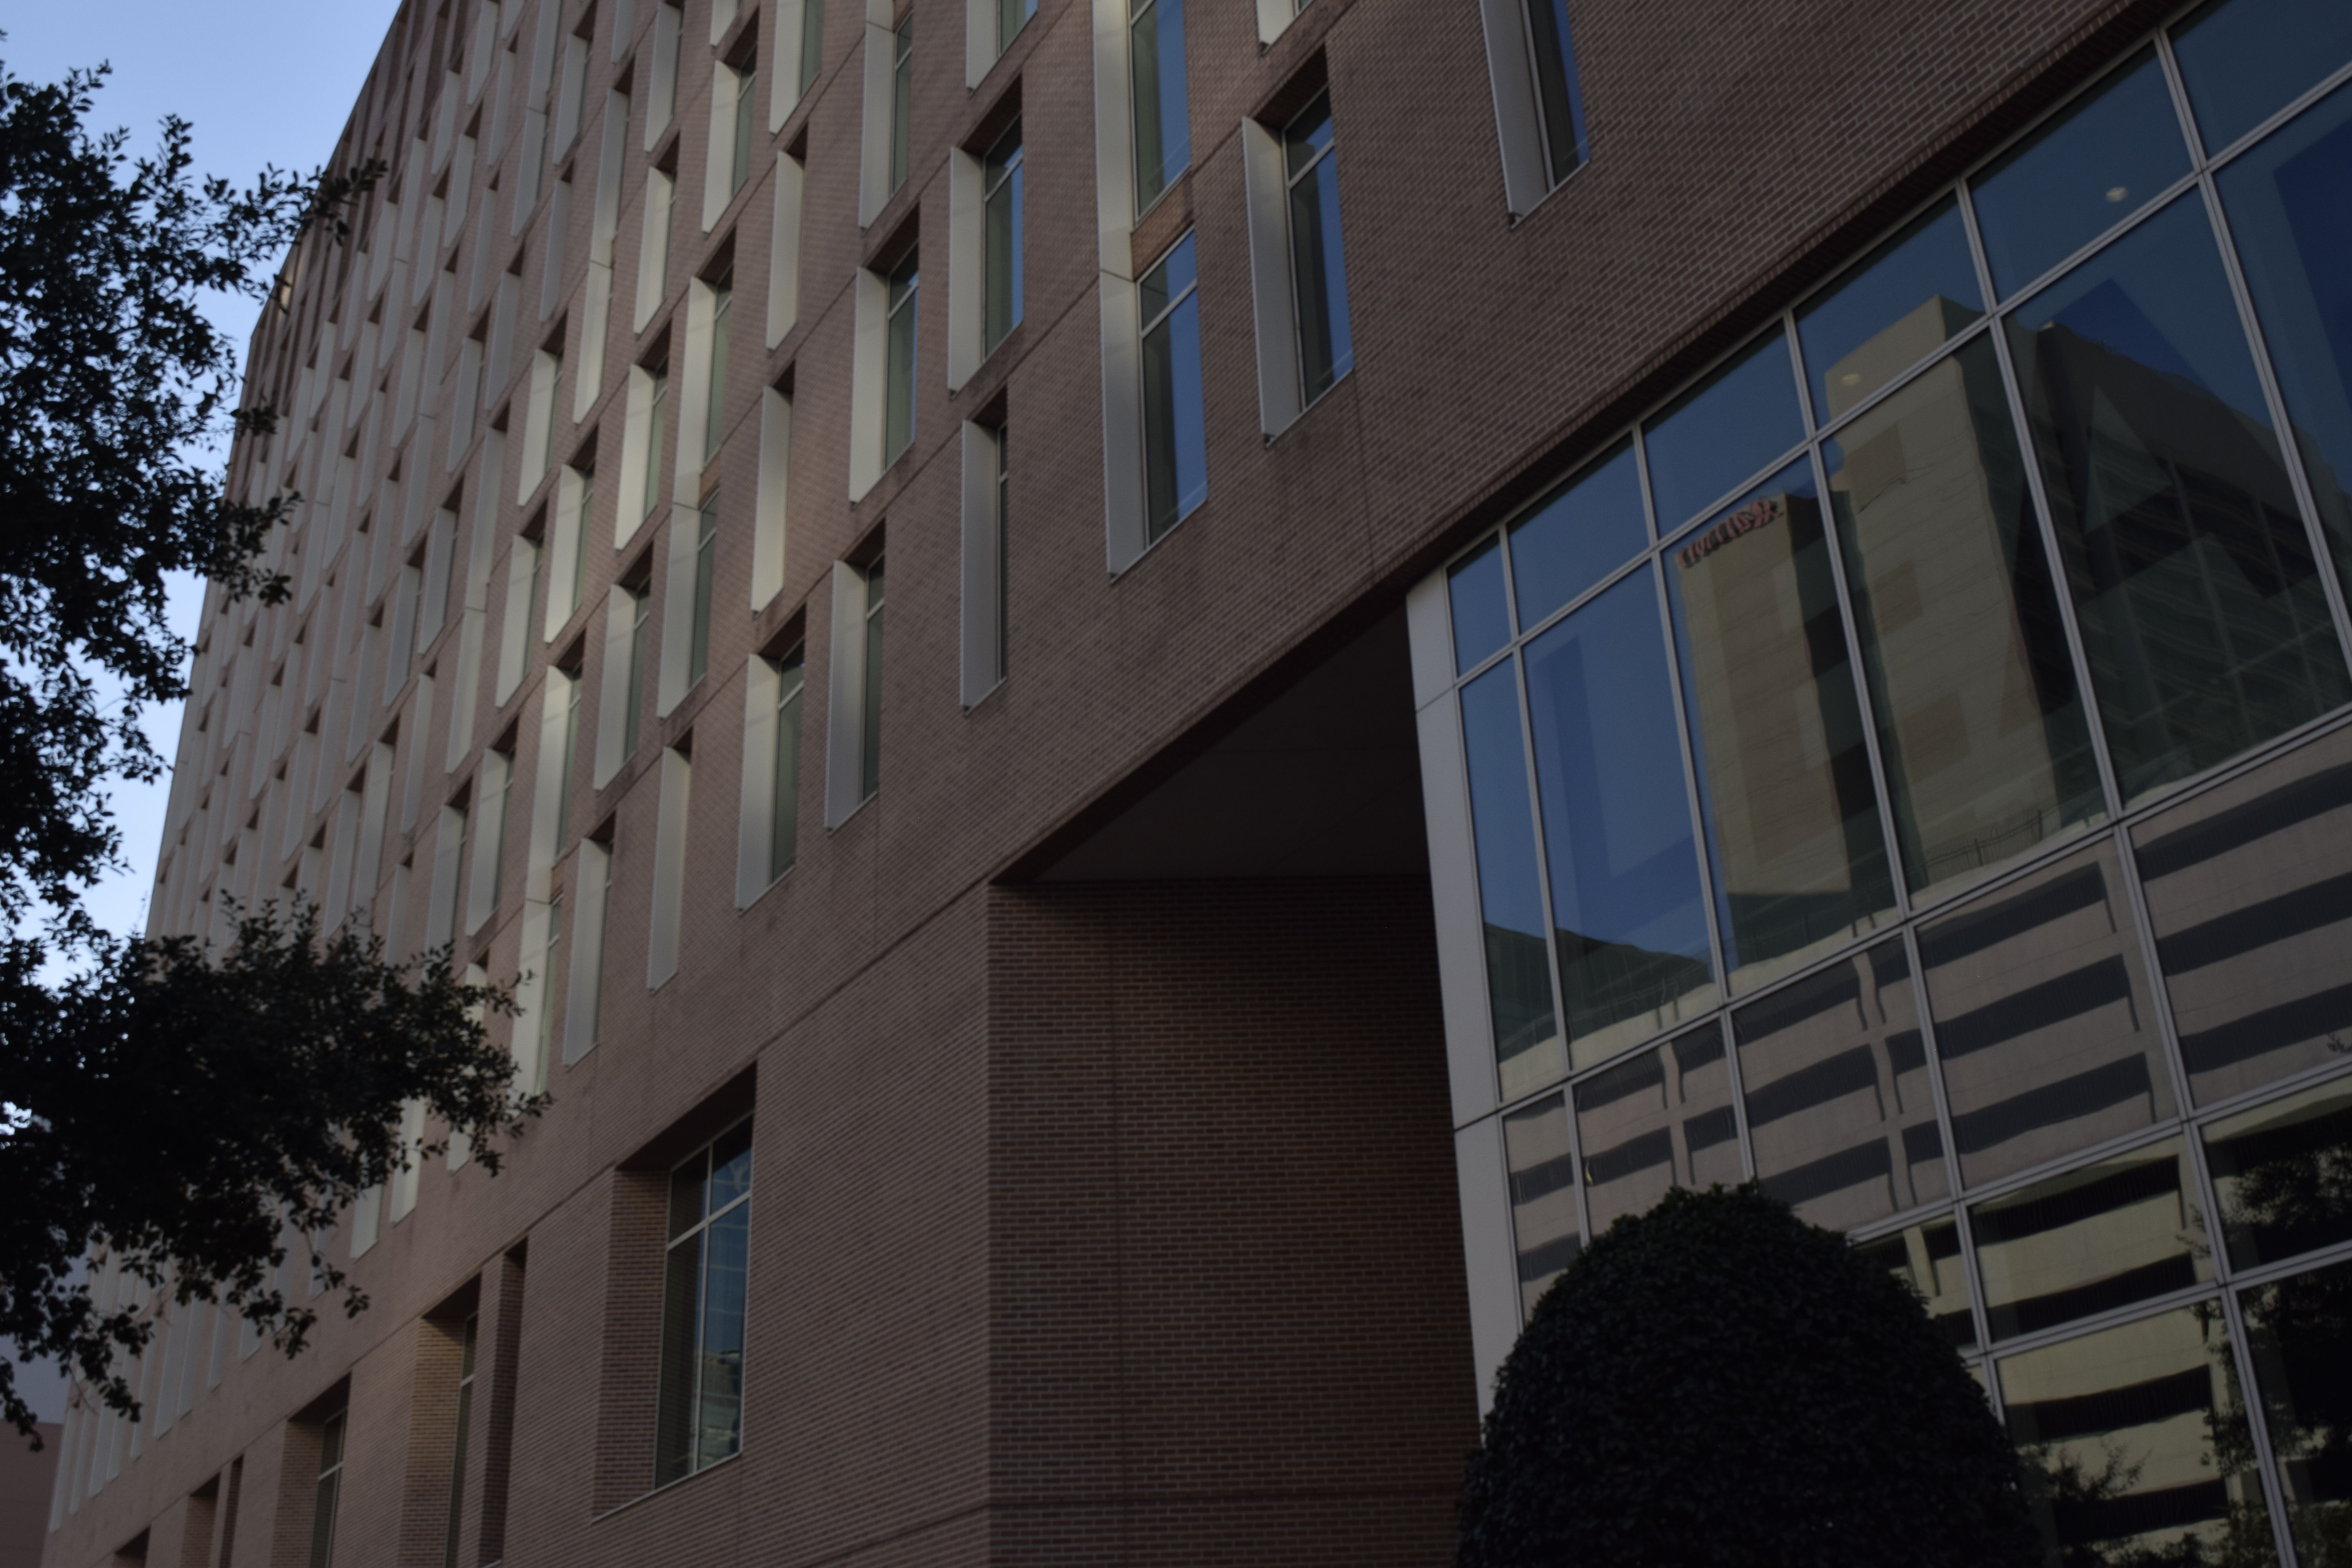
\includegraphics[width=\linewidth]{sceneA_1.jpg}
    \end{minipage}~
    \begin{minipage}{0.48\linewidth}
        \centering
        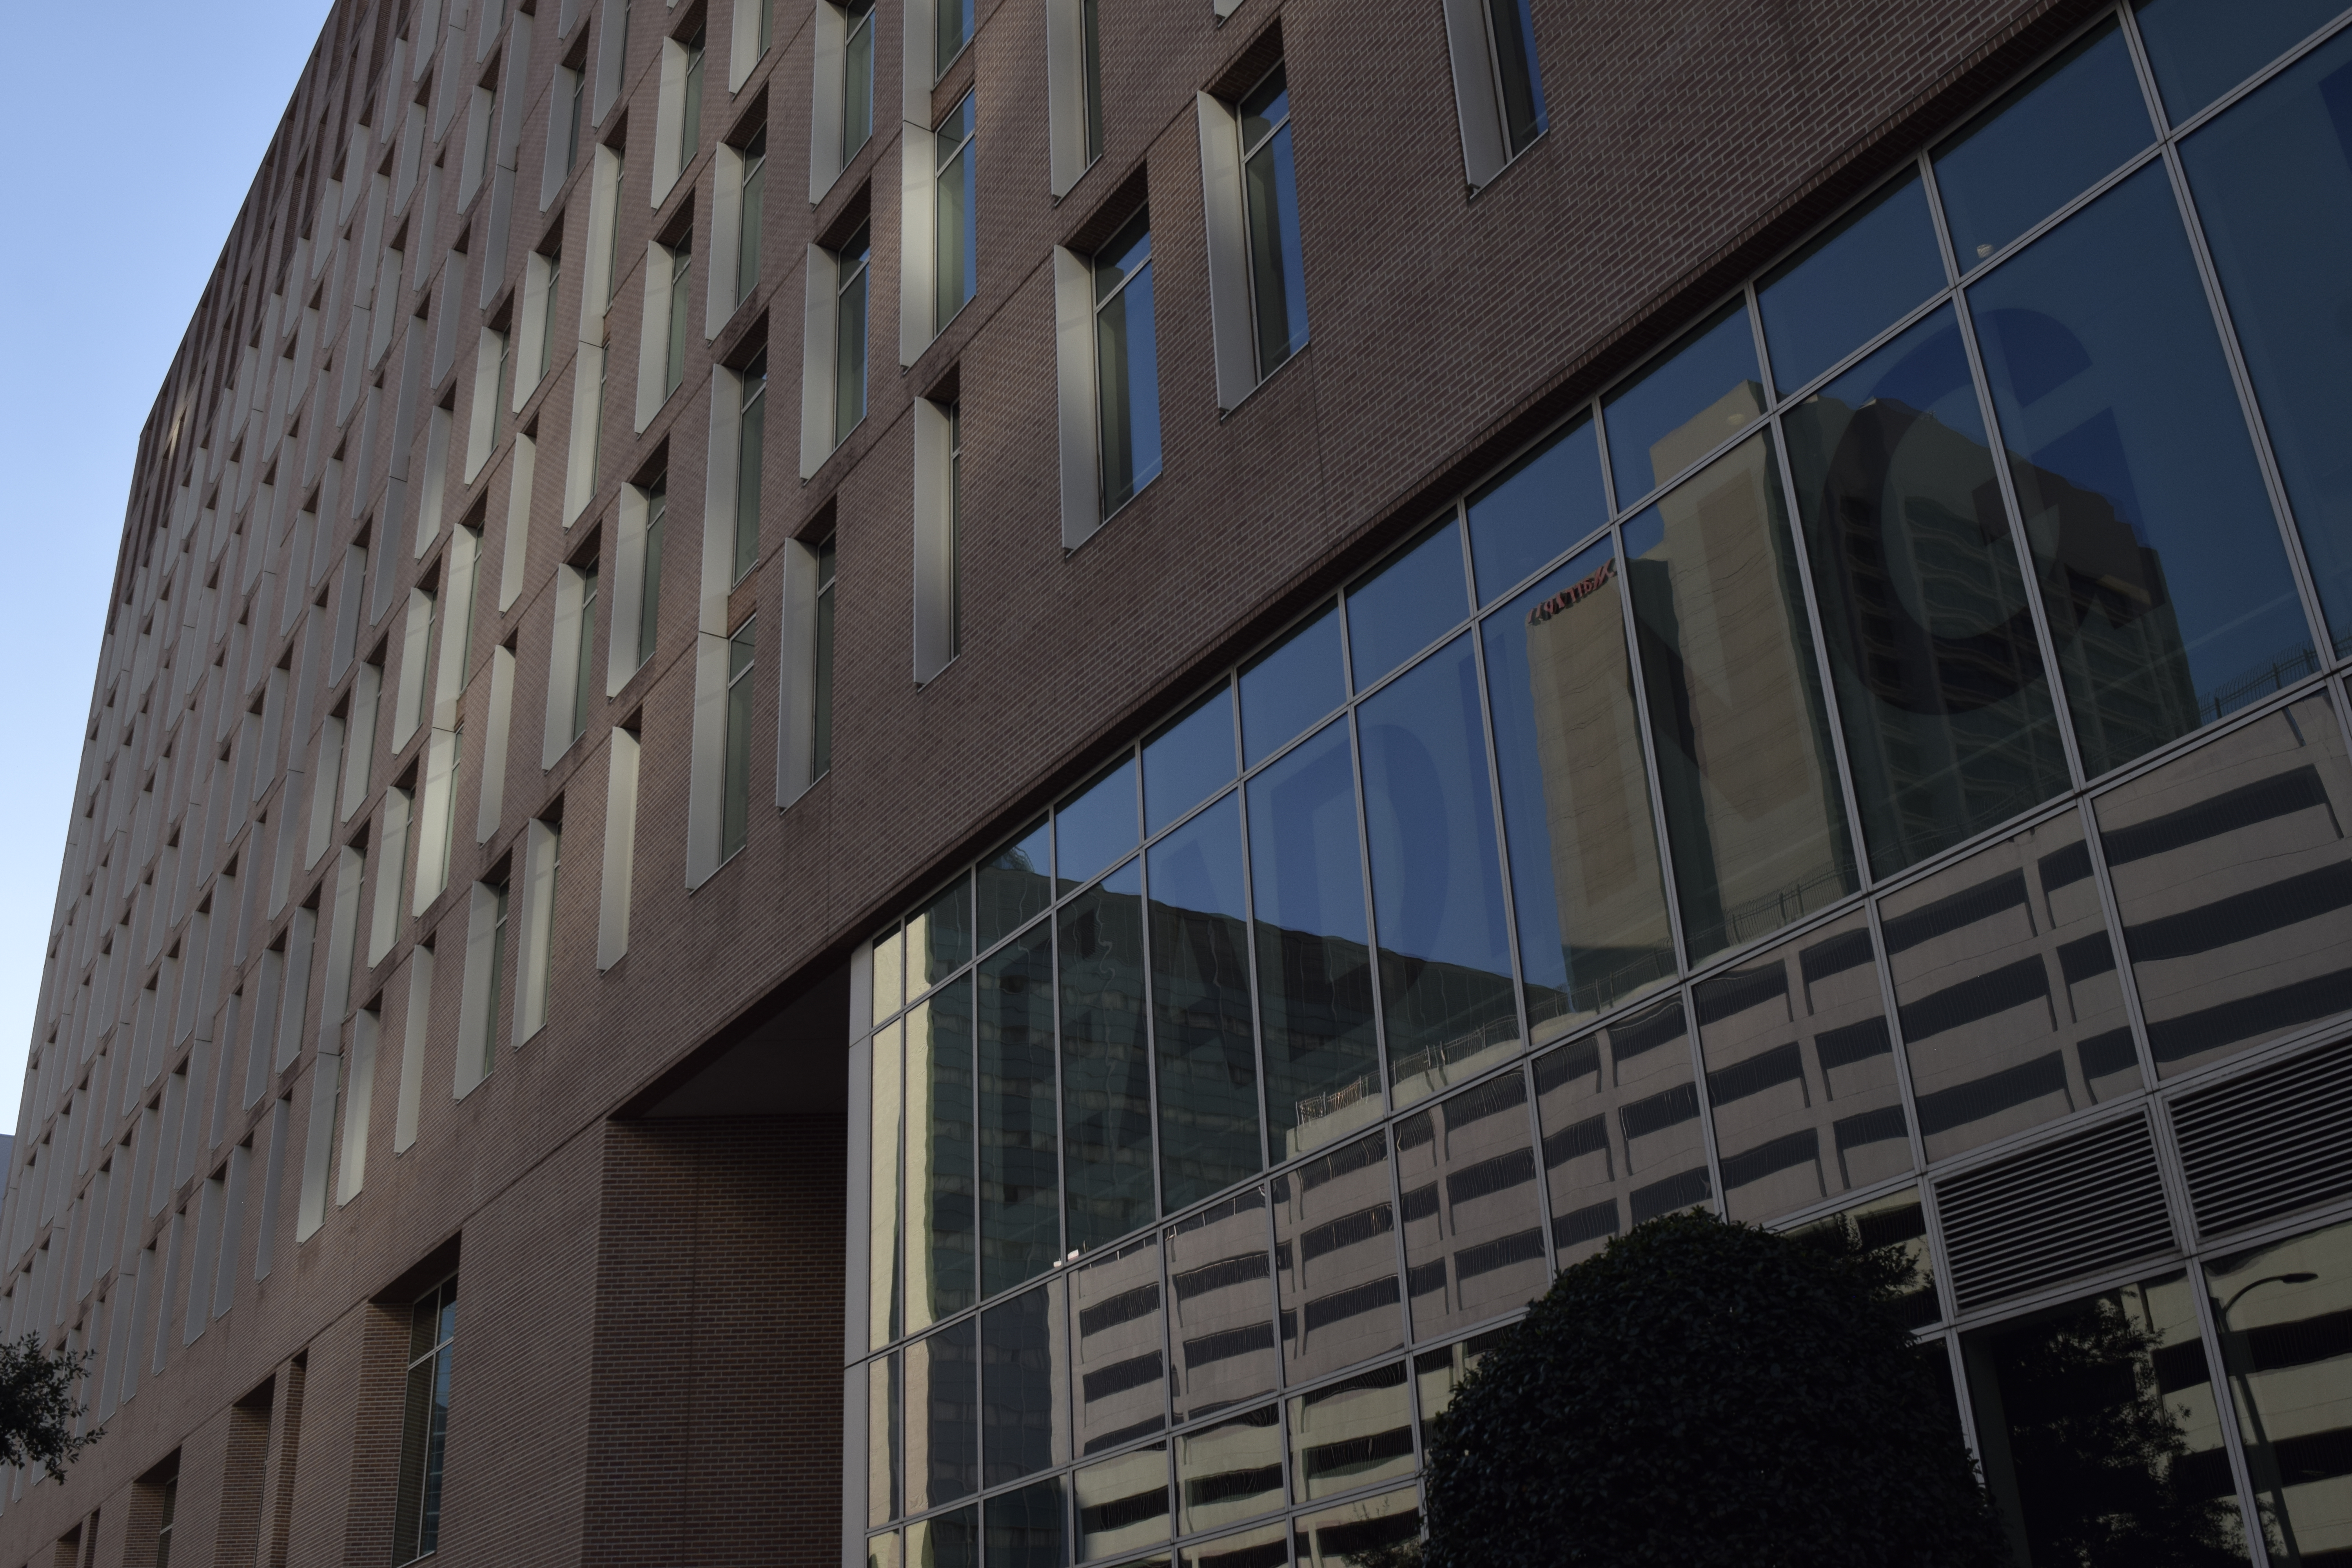
\includegraphics[width=\linewidth]{sceneA_2.jpg}
    \end{minipage}

    \vspace{3pt}

    % Row 2
    \begin{minipage}{0.48\linewidth}
        \centering
        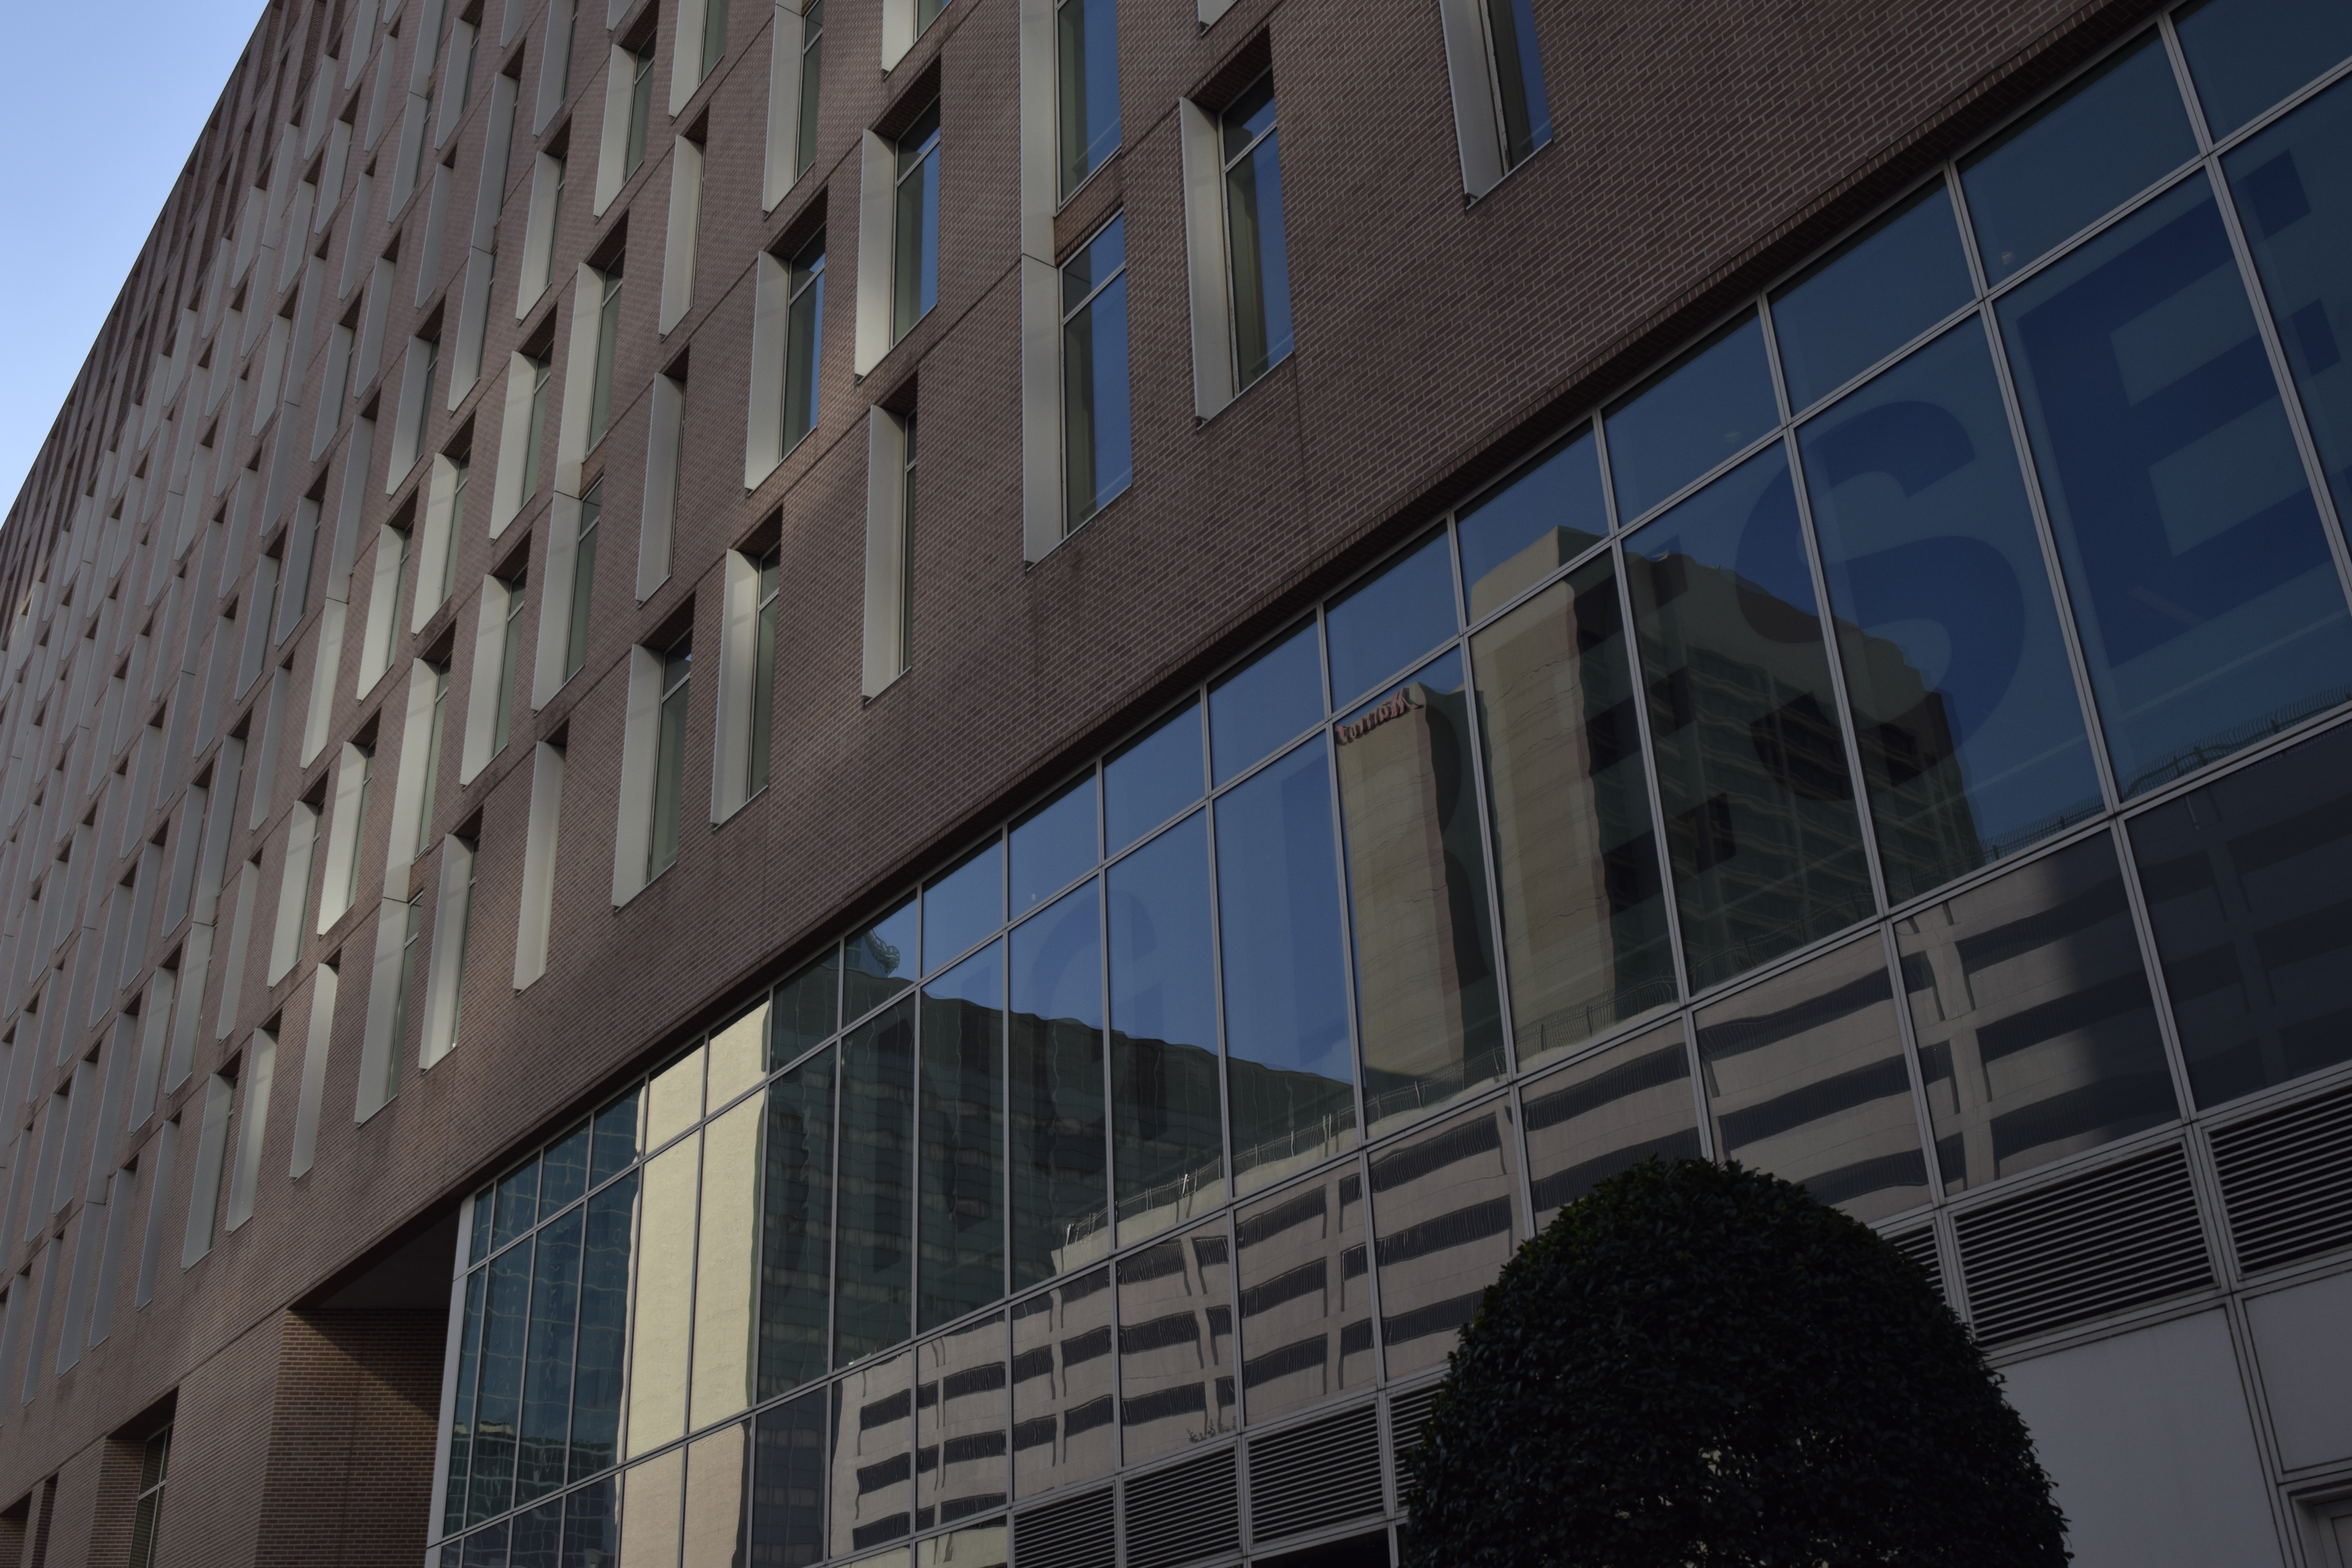
\includegraphics[width=\linewidth]{sceneA_3.jpg}
    \end{minipage}~
    \begin{minipage}{0.48\linewidth}
        \centering
        \includegraphics[width=\linewidth]{sceneA_colmap_overview.png}
    \end{minipage}

    \caption{Representative reflection sequence with sufficient non-glass anchors. 
(a)--(c) Three sampled frames from the real-world capture, showing stable lateral motion and consistent reflection structure. 
(d) Corresponding COLMAP sparse reconstruction and recovered camera trajectory.}
    \label{fig:goodcase}
\end{figure}

\subsubsection{Baseline COLMAP Facade Reconstruction}
\label{sec:colmap_baseline}

We use COLMAP as a standard SfM baseline, applying SIFT extraction, sequential matching, and incremental mapping on each sequence (e.g., DSC0036). Camera intrinsics are initialized from a chessboard calibration, with optional refinement of focal length and radial distortion. Rather than reporting global metrics, we provide representative success and failure cases in Figs.~\ref{fig:goodcase}. Sequences with sufficient non-glass texture generally reconstruct at the sparse level, while glass-dominant scenes often fragment or fail to register.

COLMAP outputs world-to-camera transforms; camera poses for visualization are obtained by inverting these transforms. We export poses and sparse points using model converter and inspect trajectories in Blender.

Qualitatively, COLMAP performs well on facades containing stable texture anchors but struggles on reflective or repetitive glass regions, producing ghost geometry and unstable trajectories. These limitations motivate incorporating a dedicated glass-segmentation module (GEM) to isolate reflective areas before reconstruction.

\subsubsection{GEM Glass Segmentation Results}
\label{sec:gem_result}

We applied GEM \cite{hao2025gem} to our collected façade sequences to identify glass regions for subsequent reflection-aware processing. GEM leverages foundation models (SAM and Grounding DINO) to produce accurate glass masks without task-specific training, making it well-suited for diverse urban glass surfaces.

% \textbf{Segmentation Performance.} 
Figure~\ref{fig:gem_results} shows a segmentation result on BRC façade sequences. GEM successfully delineates glass regions under challenging conditions, including varying lighting and complex reflections. The method achieves high precision in distinguishing glass from adjacent non-reflective surfaces such as concrete frames and metal fixtures.

\begin{figure}[!h]
  \centering
  \includegraphics[width=0.48\linewidth]{gem_input_example.png}~
  \includegraphics[width=0.48\linewidth]{gem_mask_example.png}
  \caption{GEM glass segmentation results. Left: input image from façade sequence. Right: predicted glass mask (glass regions in red).}
  \label{fig:gem_results}
\end{figure}



\subsection{Simulated Data Generation}
\begin{figure*}
    \centering
    \includegraphics[width=0.75\linewidth]{Figs/DataGenerationPipeline.png}
    \caption{Overview of our data generation pipeline. We select 3D assets and scene backgrounds, place either a flat or bumpy mirror into the scene, sample camera viewpoints, and render RGB images together with depth, normals, and albedo using Mitsuba 3.}
    \label{fig:placeholder}
\end{figure*}

Our pipeline is structured similarly to SynMirror~\cite{dhiman2025reflectingrealityenablingdiffusion} but extends the asset and scene diversity. We source 3D objects from Objaverse~\cite{objaverseXL}, ABO~\cite{collins2022abodatasetbenchmarksrealworld}, and additionally incorporate Replica scenes to introduce realistic indoor layouts and lighting. Objaverse objects are taken from the OBJECT 3DIT~\cite{michel2023object3ditlanguageguided3daware} filtered subset, and we further remove assets with invalid material behavior to ensure physically correct reflections. ABO objects are included completely for broader variation.

For scene composition, we place either a flat mirror or a procedurally generated bumpy mirror. Objects are normalized, positioned at a fixed distance from the mirror, and randomly rotated. Replica scenes or HDRI environments serve as backgrounds, while optional floor or wall textures provide additional variation.

We then sample multiple camera viewpoints around the object–mirror setup. Using Mitsuba 3, we render RGB images together with depth, surface normals, and albedo. This produces a compact and clean dataset with controlled reflection conditions and consistent geometric supervision.


\subsubsection{Simulated Normal Map Evaluation}

 \begin{figure}[htbp]
    \centering
    % Left: simulated reflection frames
    \includegraphics[width=0.46\linewidth]{frames.png}
    \hfill
    % Right: computed normal map
    \includegraphics[width=0.46\linewidth]{Normal Map.png}
    \caption{Simulated reflection sequence and corresponding normal map generated in Mitsuba~3. 
    The left image shows representative frames from a moving-camera reflection simulation, where the reflection of a straight line gradually becomes curved due to local surface normal variations. 
    The right image presents the computed color-coded normal map, with RGB channels corresponding to $(n_x,n_y,n_z)$, showing smooth orientation changes consistent with the applied surface deformation.}
    \label{fig:sim_reflection_and_normals}
\end{figure}

To validate our normal computation process, we simulated a reflective rectangular patch in Mitsuba~3 with a slightly distorted planar surface. A virtual linear light source and a moving camera were used to generate a sequence of reflected images. Figure~\ref{fig:sim_reflection_and_normals} shows several representative frames from the simulated video (left) and the corresponding color-coded normal map (right). The reflection of the straight line progressively curves as the viewing angle changes due to local surface normal variations.

The RGB channels, respectively, represent the $x$, $y$, and $z$ components of the normalized surface normals. The smooth sinusoidal pattern visible in the map reflects the intended surface deformation, confirming that the simulated scene accurately reproduces the reflective distortion characteristics of nearly flat glass surfaces as described by Jacquet \textit{et al.}~\cite{jacquet2013real}.

\subsubsection{3D Reconstruction from NeRF}

We simulated a complex classroom environment and placed either a flat mirror or a distorted mirror inside the scene. A moving camera was used to capture approximately 90 frames of mirror reflections, and these images were then fed into NeRF for reconstruction. The resulting point clouds are shown in Figure~\ref{fig:nerf}.

In the top result (flat mirror), NeRF successfully reconstructs portions of the reflected desk structure within the mirror region. This indicates that NeRF does possess a certain level of inference capability for mirror-based 3D reconstruction.

However, the bottom result (distorted mirror) shows that the entire mirror region collapses into a highly distorted and incoherent point cloud. This is because the distorted mirror introduces strong, spatially varying nonlinear mappings, breaking the geometric consistency that NeRF relies on. As a result, standard NeRF models struggle significantly with complex reflective surfaces of this kind.

\begin{figure}[htbp]
    \centering
    
    % Top image: Flat mirror NeRF result
    \includegraphics[width=0.85\linewidth]{Nerf_flatMirror.png}
    \vspace{6pt}
    
    % Bottom image: Distorted mirror NeRF result
    \includegraphics[width=0.85\linewidth]{Nerf_distortedMirror.png}

    \caption{NeRF reconstruction results in a complex simulated environment. 
    Top: NeRF reconstruction from flat-mirror reflections. 
    Bottom: NeRF reconstruction from distorted-mirror reflections.}
    \label{fig:nerf}
\end{figure}
 


\section{Discussion}
The results demonstrate clear limitations in traditional pipelines like COLMAP on glass-dominated urban facades, where reflections violate photoconsistency and produce ghost geometry or registration failures. GEM provides robust, zero-shot glass segmentation across varied conditions, supplying essential spatial priors for targeted reflection handling.

Simulations in Mitsuba confirm that distorted reflections from near-planar surfaces encode recoverable normal information, while NeRF experiments reveal the breakdown of standard neural representations under spatially varying mappings. The VGGT-based plane correction successfully restores physical mirror geometry from virtual predictions using boundary aggregation and vertical constraints.

These components establish a viable foundation. The primary remaining challenge is scale and data diversity. We will prioritize collecting extensive real-world sequences paired with the synthetic pipeline to train efficient, reflection-exploiting models that integrate into established reconstruction frameworks.

\section{Acknowledgements}
We would like to thank Professor Vivek Boominathan for his valuable guidance and feedback throughout this project. We also acknowledge the computational resources provided by Rice University that supported our simulation and model training efforts. Special thanks to the open-source communities behind GEM, COLMAP, Mitsuba, and other tools that formed the foundation of our research framework.

\section{Credit Author Statement}
Shin Li: Writing – original draft preparation, abstract and introduction; investigation.

Wentao Jiang: Experiment - Nikon D3300 DSLR Calibration, Reflection Data Collection (façade), Colmap Pose Estimation Results in Colmap and Preliminary baseline.
  
Yunan Wang: wrote the manuscript (introduction – related work, method, and results for normal map); methodology design; simulation and analysis of reflective surface normal estimation using Mitsuba~3.

Chi Xu: Writing the Colmap part in Methods and the Acknowledgments section. Implement the pipeline of simulation from captured video to 3D scenes through Colmap and apply the GEM glass segmentation model. 

Yixing Liu: Designing and implementing the VGGT-Based Mirror Correction method and presenting resutls, using Mitsuba 3 to render scenes to get simulated data, writing the corresponding part in the report.
% Keep your text and graphic files separate until after the text has been 
% formatted and styled. Do not number text heads---{\LaTeX} will do that 
% for you.

% \subsection{Abbreviations and Acronyms}\label{AA}
% Define abbreviations and acronyms the first time they are used in the text, 
% even after they have been defined in the abstract. Abbreviations such as 
% IEEE, SI, MKS, CGS, ac, dc, and rms do not have to be defined. Do not use 
% abbreviations in the title or heads unless they are unavoidable.

% \subsection{Units}
% \begin{itemize}
% \item Use either SI (MKS) or CGS as primary units. (SI units are encouraged.) English units may be used as secondary units (in parentheses). An exception would be the use of English units as identifiers in trade, such as ``3.5-inch disk drive''.
% \item Avoid combining SI and CGS units, such as current in amperes and magnetic field in oersteds. This often leads to confusion because equations do not balance dimensionally. If you must use mixed units, clearly state the units for each quantity that you use in an equation.
% \item Do not mix complete spellings and abbreviations of units: ``Wb/m\textsuperscript{2}'' or ``webers per square meter'', not ``webers/m\textsuperscript{2}''. Spell out units when they appear in text: ``. . . a few henries'', not ``. . . a few H''.
% \item Use a zero before decimal points: ``0.25'', not ``.25''. Use ``cm\textsuperscript{3}'', not ``cc''.)
% \end{itemize}

% \subsection{Equations}
% Number equations consecutively. To make your 
% equations more compact, you may use the solidus (~/~), the exp function, or 
% appropriate exponents. Italicize Roman symbols for quantities and variables, 
% but not Greek symbols. Use a long dash rather than a hyphen for a minus 
% sign. Punctuate equations with commas or periods when they are part of a 
% sentence, as in:
% \begin{equation}
% a+b=\gamma\label{eq}
% \end{equation}

% Be sure that the 
% symbols in your equation have been defined before or immediately following 
% the equation. Use ``\eqref{eq}'', not ``Eq.~\eqref{eq}'' or ``equation \eqref{eq}'', except at 
% the beginning of a sentence: ``Equation \eqref{eq} is . . .''

% \subsection{\LaTeX-Specific Advice}

% Please use ``soft'' (e.g., \verb|\eqref{Eq}|) cross references instead
% of ``hard'' references (e.g., \verb|(1)|). That will make it possible
% to combine sections, add equations, or change the order of figures or
% citations without having to go through the file line by line.

% Please don't use the \verb|{eqnarray}| equation environment. Use
% \verb|{align}| or \verb|{IEEEeqnarray}| instead. The \verb|{eqnarray}|
% environment leaves unsightly spaces around relation symbols.

% Please note that the \verb|{subequations}| environment in {\LaTeX}
% will increment the main equation counter even when there are no
% equation numbers displayed. If you forget that, you might write an
% article in which the equation numbers skip from (17) to (20), causing
% the copy editors to wonder if you've discovered a new method of
% counting.

% {\BibTeX} does not work by magic. It doesn't get the bibliographic
% data from thin air but from .bib files. If you use {\BibTeX} to produce a
% bibliography you must send the .bib files. 

% {\LaTeX} can't read your mind. If you assign the same label to a
% subsubsection and a table, you might find that Table I has been cross
% referenced as Table IV-B3. 

% {\LaTeX} does not have precognitive abilities. If you put a
% \verb|\label| command before the command that updates the counter it's
% supposed to be using, the label will pick up the last counter to be
% cross referenced instead. In particular, a \verb|\label| command
% should not go before the caption of a figure or a table.

% Do not use \verb|\nonumber| inside the \verb|{array}| environment. It
% will not stop equation numbers inside \verb|{array}| (there won't be
% any anyway) and it might stop a wanted equation number in the
% surrounding equation.

% \subsection{Some Common Mistakes}\label{SCM}
% \begin{itemize}
% \item The word ``data'' is plural, not singular.
% \item The subscript for the permeability of vacuum $\mu_{0}$, and other common scientific constants, is zero with subscript formatting, not a lowercase letter ``o''.
% \item In American English, commas, semicolons, periods, question and exclamation marks are located within quotation marks only when a complete thought or name is cited, such as a title or full quotation. When quotation marks are used, instead of a bold or italic typeface, to highlight a word or phrase, punctuation should appear outside of the quotation marks. A parenthetical phrase or statement at the end of a sentence is punctuated outside of the closing parenthesis (like this). (A parenthetical sentence is punctuated within the parentheses.)
% \item A graph within a graph is an ``inset'', not an ``insert''. The word alternatively is preferred to the word ``alternately'' (unless you really mean something that alternates).
% \item Do not use the word ``essentially'' to mean ``approximately'' or ``effectively''.
% \item In your paper title, if the words ``that uses'' can accurately replace the word ``using'', capitalize the ``u''; if not, keep using lower-cased.
% \item Be aware of the different meanings of the homophones ``affect'' and ``effect'', ``complement'' and ``compliment'', ``discreet'' and ``discrete'', ``principal'' and ``principle''.
% \item Do not confuse ``imply'' and ``infer''.
% \item The prefix ``non'' is not a word; it should be joined to the word it modifies, usually without a hyphen.
% \item There is no period after the ``et'' in the Latin abbreviation ``et al.''.
% \item The abbreviation ``i.e.'' means ``that is'', and the abbreviation ``e.g.'' means ``for example''.
% \end{itemize}
% An excellent style manual for science writers is \cite{b7}.

% \subsection{Authors and Affiliations}
% \textbf{The class file is designed for, but not limited to, six authors.} A 
% minimum of one author is required for all conference articles. Author names 
% should be listed starting from left to right and then moving down to the 
% next line. This is the author sequence that will be used in future citations 
% and by indexing services. Names should not be listed in columns nor group by 
% affiliation. Please keep your affiliations as succinct as possible (for 
% example, do not differentiate among departments of the same organization).

% \subsection{Identify the Headings}
% Headings, or heads, are organizational devices that guide the reader through 
% your paper. There are two types: component heads and text heads.

% Component heads identify the different components of your paper and are not 
% topically subordinate to each other. Examples include Acknowledgments and 
% References and, for these, the correct style to use is ``Heading 5''. Use 
% ``figure caption'' for your Figure captions, and ``table head'' for your 
% table title. Run-in heads, such as ``Abstract'', will require you to apply a 
% style (in this case, italic) in addition to the style provided by the drop 
% down menu to differentiate the head from the text.

% Text heads organize the topics on a relational, hierarchical basis. For 
% example, the paper title is the primary text head because all subsequent 
% material relates and elaborates on this one topic. If there are two or more 
% sub-topics, the next level head (uppercase Roman numerals) should be used 
% and, conversely, if there are not at least two sub-topics, then no subheads 
% should be introduced.

% \subsection{Figures and Tables}
% \paragraph{Positioning Figures and Tables} Place figures and tables at the top and 
% bottom of columns. Avoid placing them in the middle of columns. Large 
% figures and tables may span across both columns. Figure captions should be 
% below the figures; table heads should appear above the tables. Insert 
% figures and tables after they are cited in the text. Use the abbreviation 
% ``Fig.~\ref{fig}'', even at the beginning of a sentence.

% \begin{table}[htbp]
% \caption{Table Type Styles}
% \begin{center}
% \begin{tabular}{|c|c|c|c|}
% \hline
% \textbf{Table}&\multicolumn{3}{|c|}{\textbf{Table Column Head}} \\
% \cline{2-4} 
% \textbf{Head} & \textbf{\textit{Table column subhead}}& \textbf{\textit{Subhead}}& \textbf{\textit{Subhead}} \\
% \hline
% copy& More table copy$^{\mathrm{a}}$& &  \\
% \hline
% \multicolumn{4}{l}{$^{\mathrm{a}}$Sample of a Table footnote.}
% \end{tabular}
% \label{tab1}
% \end{center}
% \end{table}

% \begin{figure}[htbp]
% \centerline{\includegraphics{fig1.png}}
% \caption{Example of a figure caption.}
% \label{fig}
% \end{figure}

% Figure Labels: Use 8 point Times New Roman for Figure labels. Use words 
% rather than symbols or abbreviations when writing Figure axis labels to 
% avoid confusing the reader. As an example, write the quantity 
% ``Magnetization'', or ``Magnetization, M'', not just ``M''. If including 
% units in the label, present them within parentheses. Do not label axes only 
% with units. In the example, write ``Magnetization (A/m)'' or ``Magnetization 
% \{A[m(1)]\}'', not just ``A/m''. Do not label axes with a ratio of 
% quantities and units. For example, write ``Temperature (K)'', not 
% ``Temperature/K''.

% \section*{Acknowledgment}

\newpage
\bibliographystyle{IEEEtran}
\bibliography{ref}



\end{document}
